%!TEX root = ../../main.tex


\begin{figure}[!htb]
\centering
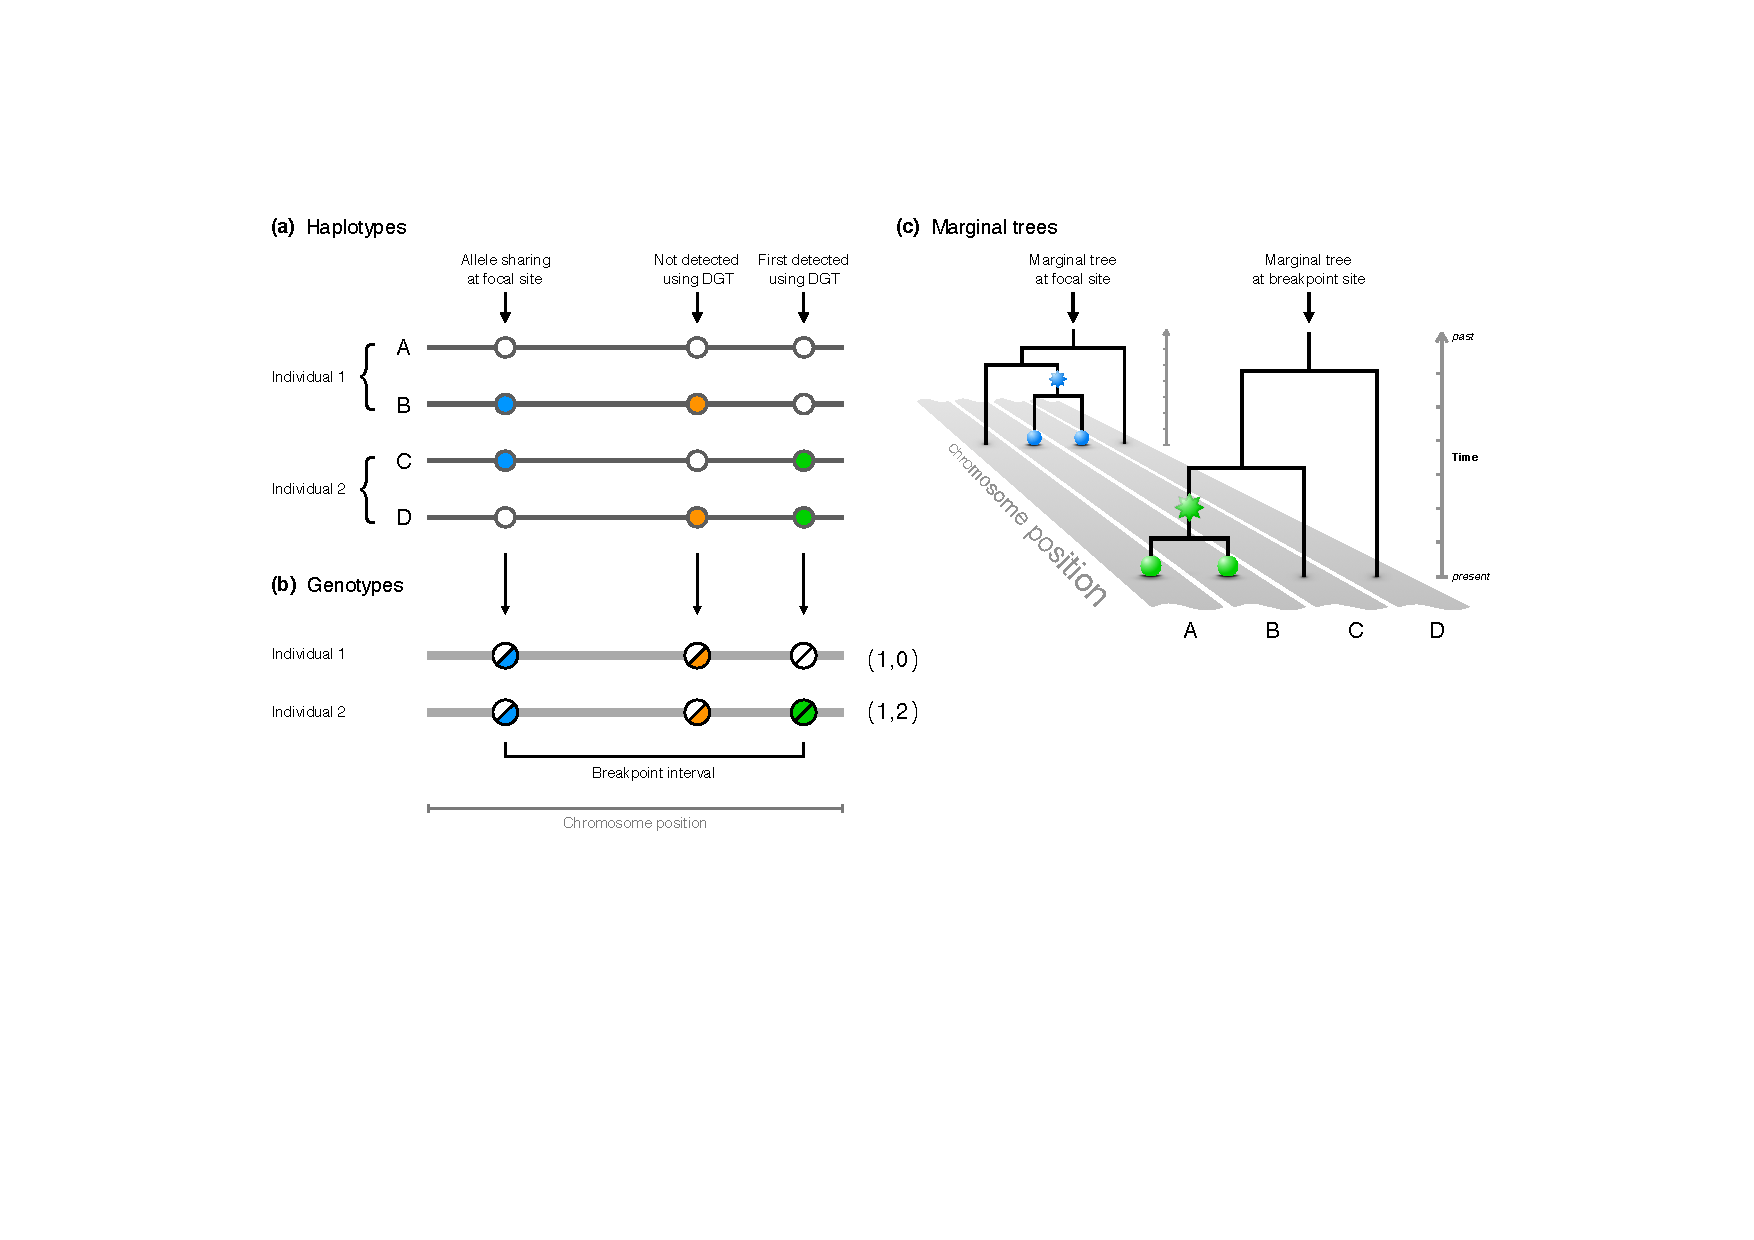
\includegraphics[width=\textwidth]{./img/ch3/info_dgt_new}
\Caption{Breakpoint detection using the discordant genotype test (DGT)}
{Unlike the \gls{fgt}, which requires haplotype information, the \gls{dgt} identifies a breakpoint interval using genotype data.
This representation extends the example shown for the \gls{fgt} in \cpref{fig:info_fgt}.
For comparison, Panel~\textbf{(a)} shows the \n{4} gametes of the \n{2} individuals involved.
Panel~\textbf{(b)} shows the \n{2} corresponding genotype sequences per individual (\emph{thick} horizontal lines) from which a breakpoint interval is inferred using the \gls{dgt}.
The genotypic states of the breakpoint sites are given on the \emph{right}.
Genotypes can either be homozygous for the ancestral allele (\emph{hollow} circle), heterozygous (\emph{semi-solid}), or homozygous for the derived allele (\emph{solid}).
The site indicated between the focal site and the detected breakpoint would satisfy the breakpoint condition under the \gls{fgt}, but is missed under the \gls{dgt}.
Panel~\textbf{(c)} shows the corresponding marginal trees at the focal site and the detected breakpoint, where \emph{stars} indicate a mutation event and \emph{spheres} the derived alleles.}
{fig:info_dgt}
\end{figure}
